\newcommand{\department}{Физики}
\newcommand{\labnum}{16}
\newcommand{\discipline}{Физика}
\newcommand{\theme}{ИЗМЕРЕНИЕ МАГНИТНОГО ПОЛЯ ЗЕМЛИ}
\newcommand{\haspartner}{0} % 0 or 1
\newcommand{\partnername}{}
\newcommand{\teachername}{Лоскутников В.С.}
\newcommand{\labyear}{2020}

\documentclass[12pt,a4paper]{article}  % шаблон для статьи, шрифт 12 пт

\usepackage[utf8]{inputenc}  % использование кодировки Юникод UTF-8
\usepackage[T1]{fontenc}
\usepackage[russian]{babel}  % пакет поддержки русского языка

\usepackage{indentfirst}  % отступ первого абзаца
\setlength{\parindent}{0.75cm}

\usepackage[compact]{titlesec}  % для titlespacing
% \titlespacing{\заголовок}{слева}{перед}{после}[справа]
\titlespacing*{\section}{0.75cm}{1em}{0.1em}  % отступ заголовка
\titlespacing*{\subsection}{0.75cm}{1em}{0.1em}


\usepackage{graphicx}  % кртинки
\usepackage{float} % плавающие картинки
\usepackage{wrapfig}  % Обтекание фигур (таблиц, картинок и прочего)
\usepackage[labelsep=endash]{caption}  % тире вместо двоеточия в картинках
\usepackage{amsmath}




\begin{document}

	\thispagestyle{empty}

\begin{center}
    \Large{
    \textbf{МИНОБРНАУКИ РОССИИ}

    \textbf{Санкт-Петербургский государственный}

    \textbf{электротехнический университет «ЛЭТИ»}

    \textbf{им. В.И. Ульянова (Ленина)}

    \textbf{Кафедра \department}
    }
\end{center}

\topskip=0pt
\vspace*{\fill}

\begin{center}
    \Large{
    \textbf{
    ЛАБОРАТОРНАЯ РАБОТА №\labnum\\
    по дисциплине «\discipline»\\
    Тема: \theme\\
    }
    }
\end{center}

\vspace*{\fill}

\begin{tabular}{lcr}
    Студент \if \haspartner 1ы \fi \ гр. 9892 & \begin{tabular}{p{60mm}} \\ \hline \end{tabular} & Лескин К.А.  \\\\
    \if \haspartner 1
                      & \begin{tabular}{p{60mm}} \\ \hline \end{tabular} & \partnername \\\\
    \fi
    Преподаватель     & \begin{tabular}{p{60mm}} \\ \hline \end{tabular} & \teachername
    \\\\
\end{tabular}

\begin{center}
    Санкт-Петербург\\
    \labyear
\end{center}

\newpage
	
	\section*{Цель}

Изучение действия магнитного поля на движущиеся заряды в полупроводнике, с
электронным типом проводимости, определение постоянной Холла, концентрации и подвижности носителей
заряда. 


	\section*{Приборы и принадлежности}

Установка для исследования эффекта Холла включает:

\begin{itemize}
	\item датчик Холла \textbf{ДХ}, выполненный в виде пленки, напыленной на подложку из диэлектрика с четырьмя электродами для подведения электрического тока и измерения разности потенциалов Холла;
	\item электромагнит \textbf{ЭМ-} состоящий из соосной системы двух круговых катушек с током, расположенных на
	сердечнике из магнитомягкого материала;
	\item источников питания $ E_1 $ и $ E_2 $;
	\item потенциометр $ R_1 $ «\textbf{Ток ДХ}»,регулирующий ток $ I_1 $ через \textbf{ДХ};
	\item потенциометр $ R_2 $ «\textbf{Ток ЭМ}», регулирующий ток $ I_2 $ через электромагнит \textbf{ЭМ};
	\item миллиамперметр \textbf{mA}, измеряющий ток $ I_1 $ через \textbf{ДХ};
	\item вольтметр \textbf{V}$_2$, измеряющий падение напряжения на резисторе $ R $. Поскольку сопротивление $ R = 1 $ Ом ---
	значение напряжения $ U_2 $ численно равно $ I_2 $;
	\item операционный усилитель \textbf{ОУ} с коэффициентом усиления $ k $;
	\item вольтметр \textbf{V}$_1$, измеряющий напряжение $ U_1 $ на выходе \textbf{ОУ}, пропорциональное ЭДС на выходе датчика Холла
	$ U_x $. 

\end{itemize}

\newpage

Установка представлена на рис. \ref{schema}

\begin{figure}[hpt!]
	\centering
	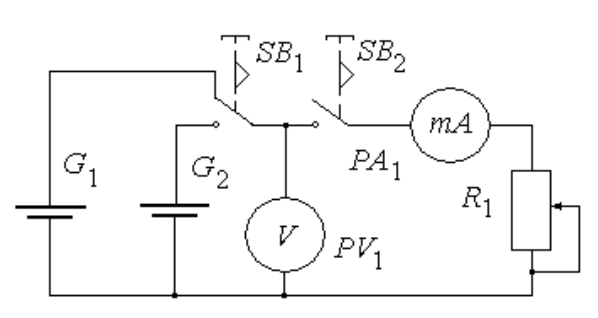
\includegraphics[width=0.8\linewidth]{photo/schema}
	\caption{Схема установки для исследования эффекта Холла}
	\label{schema}
\end{figure}


	
	\section*{Исследуемые закономерности}

\textbf{Модель электростатического поля}

В проводящей среде под
действием приложенной к электродам постоянной разности потенциалов
происходит направленное движение заряженных частиц, в результате чего в
среде, окружающей электроды, устанавливается стационарное распределение
потенциала, подобное распределению потенциала в диэлектрической среде
вокруг заряженных проводящих тел, если форма и взаимное расположение
последних аналогичны соответствующим параметрам электродов
проводящей модели. 



\begin{equation}
	F = qE = -q\dfrac{\varDelta \varphi}{\varDelta l}n,
\end{equation}

где $ n $ -- единичный вектор в направлении максимального изменения
потенциала, то в проводящей среде вектор плотности тока подчиняется
вполне симметричному соотношению 

\begin{equation}
	j = -\gamma\dfrac{\Delta\varphi}{\Delta l}n = \gamma E,
\end{equation} 

где $ \gamma $ -- электропроводность среды (величина, обратная удельному
сопротивлению). 


Из сопоставления двух соотношений видно, что:

\begin{enumerate}
	\item оба поля
	потенциальны, (не образуют вихрей в пространстве, окружающем
	электроды);
	\item как линии напряженности электростатического
	поля, так и линии тока перпендикулярны линиям или поверхностям равного
	потенциала. 
\end{enumerate} 

\textbf{Поле длинной двухпроводной линии}

На планшете моделируются поля,
картина которых остается неизменной при
параллельном переносе плоскости, в
которой исследуется поле. 

В данной работе исследуется поле двух
длинных, параллельных, равномерно и
разноименно заряженных проводящих
цилиндров (двухпроводной линии). 

Для каждого цилиндра напряженность поля равна 

\begin{equation}
	E = \dfrac{\tau}{2\pi\varepsilon\varepsilon_0r}
\end{equation}

Значение и направление результирующего вектора напряженности поля
определяют по отношению к системе координат $ x0y $, заданной
экспериментатором. 

\textbf{Напряженность поля и вектор индукции}

Для электростатического
поля справедливо следующее соотношение между вектором напряженности
поля и вектором электрической индукции

\begin{equation}\label{vec}
	D = \varepsilon\varepsilon_0E
\end{equation}

\textbf{Поток вектора индукции электрического поля (теорема Гаусса)}

Поток вектора индукции электрического поля определяется выражением

\begin{equation}
	\Phi_D = \int_S Dds = \int_S Dnds = \int_S Dds\cos(Dn) = \int_S D_n ds
\end{equation}

где $ S $ – поверхность произвольной формы в области поля; $ n $ – единичный
вектор нормали в данной точке поверхности. 

Для электростатического поля справедлива теорема Гаусса

\begin{equation}
	\oint_S Dds = \int_V \rho dV = Q_V
\end{equation}

где $ S $ – произвольная замкнутая поверхность в области поля; $ V $ – объем
области поля, ограниченный поверхностью $ S $; $ Q_V $ – заряд, распределенный в
объеме $ V $. 


Это означает, что выражение (\ref{vec}) следует понимать так: \textit{поток вектора
индукции электростатического поля через замкнутую поверхность
произвольной формы равен суммарному заряду, заключенному в объеме,
ограниченном этой поверхностью, и не зависит от зарядов, расположенных
вне данной поверхности. 
}

\textbf{Циркуляция вектора напряженности электрического поля}

В электрическом поле циркуляцией вектора напряженности
называют физическую величину, которая определяется соотношением 

\begin{equation}\label{key}
	\Gamma = \oint_L Edl = \oint_L Edl\cos(E\tau) = \oint_L E_l dl
\end{equation}

где $ L $ – произвольный замкнутый контур; $ \tau $ – единичный вектор касательной
к линии контура в данной точке. 
	
	\newpage
	
	\section*{Протокол}

\begin{tabular}{|l|c|}
	\hline
	$ i $ & $ U_\Gamma, B $ \\
	\hline
	1 & 2.6 \\
	\hline
	2 & 2.7 \\
	\hline
	3 & 2.6 \\
	\hline
	4 & 2.3 \\
	\hline
	5 & 2.5 \\
	\hline
	6 & 2.5 \\
	\hline
	7 & 2.3 \\
	\hline
	8 & 2.6 \\
	\hline
	9 & 2.3 \\
	\hline
	10 & 2.5 \\
	\hline
\end{tabular}
\quad
\begin{tabular}{|l|c|}
	\hline
	$ i $ & $ U_B, B $ \\
	\hline
	1 & 7.5 \\
	\hline
	2 & 7.2 \\
	\hline
	3 & 7.5 \\
	\hline
	4 & 7.4 \\
	\hline
	5 & 6.9 \\
	\hline
	6 & 7.2 \\
	\hline
	7 & 7.1 \\
	\hline
	8 & 7.2 \\
	\hline
	9 & 7.0 \\
	\hline
	10 & 7.4 \\
	\hline
\end{tabular}
\\
\\
\\

Константы эксперимента

\begin{tabular}{|lcr|}
	\hline
	$ r $ & радиус катушки & 100 мм\\
	$ N $ & кол-во витков & 2000\\
	$ C $ & ёмкость конденсатора & 2 мкФ\\
	$ R $ & сопротивление & 470 Ом\\
	\hline
\end{tabular}
	
	\newpage
	
	\section*{Обработка результатов измерений}

\begin{table}[htp!]
    \centering
    \label{table}
    \scalebox{1}{
        \begin{tabular}{|c|c|c|c|}
            \hline
            $ I_1 $, мА & $ I_2 = U_2 $, мА & $ U_1 $, В & $ R = \dfrac{U_x * d}{BI_{xi}} $\\
            \hline
            \multirow{7}{*}{2.0}
            & -0.1 & -0.98 & 0.3887\\
            \cline{2-4}
            & -0.2 & -1.2 & 0.23798\\
            \cline{2-4}
            & -0.3 & -1.4 & 0.1851\\
            \cline{2-4}
            & -0.4 & -1.7 & 0.16857\\
            \cline{2-4}
            & -0.5 & -1.85 & 0.14676\\
            \cline{2-4}
            & -0.6 & -2.13 & 0.14081\\
            \cline{2-4}
            & -0.7 & -2.28 & 0.12919\\
            \hline
            \multirow{7}{*}{3.0}
            & -0.1 & -1.44 & 0.56877\\
            \cline{2-4}
            & -0.2 & -1.77 & 0.34955\\
            \cline{2-4}
            & -0.3 & -2.1 & 0.27648\\
            \cline{2-4}
            & -0.4 & -2.47 & 0.2439\\
            \cline{2-4}
            & -0.5 & -2.8 & 0.22119\\
            \cline{2-4}
            & -0.6 & -3.14 & 0.2067\\
            \cline{2-4}
            & -0.7 & -3.35 & 0.18902\\
            \hline
            \multirow{7}{*}{4.0}
            & -0.1 & -1.84 & 0.72373\\
            \cline{2-4}
            & -0.2 & -2.27 & 0.44643\\
            \cline{2-4}
            & -0.3 & -2.66 & 0.34875\\
            \cline{2-4}
            & -0.4 & -3.11 & 0.30581\\
            \cline{2-4}
            & -0.5 & -3.56 & 0.28005\\
            \cline{2-4}
            & -0.6 & -4.06 & 0.26615\\
            \cline{2-4}
            & -0.7 & -4.33 & 0.2433\\
            \hline
            \multirow{7}{*}{5.0}
            & -0.1 & -2.27 & 0.88915\\
            \cline{2-4}
            & -0.2 & -2.75 & 0.53858\\
            \cline{2-4}
            & -0.3 & -3.3 & 0.43087\\
            \cline{2-4}
            & -0.4 & -3.88 & 0.37995\\
            \cline{2-4}
            & -0.5 & -4.49 & 0.35174\\
            \cline{2-4}
            & -0.6 & -5.0 & 0.32641\\
            \cline{2-4}
            & -0.7 & -5.41 & 0.30273\\
            \hline
            \multirow{7}{*}{6.0}
            & -0.1 & -2.68 & 1.0454\\
            \cline{2-4}
            & -0.2 & -3.34 & 0.65143\\
            \cline{2-4}
            & -0.3 & -4.0 & 0.5201\\
            \cline{2-4}
            & -0.4 & -4.6 & 0.44859\\
            \cline{2-4}
            & -0.5 & -5.37 & 0.41894\\
            \cline{2-4}
            & -0.6 & -5.84 & 0.37967\\
            \cline{2-4}
            & -0.7 & -6.4 & 0.35664\\
            \hline
            
        \end{tabular}
    }  % scalebox
\end{table}


\newpage

Рассчитаем среднее значение и доверительную погрешность $ R_x $:\\

% выборочное среднее
$ 
\overline{R_{x}}= 
\sum_{i=1}^{35} R_{xi} = 
\dfrac{0.3887}{35} + 
\dfrac{0.23798}{35} + 
\dfrac{0.1851}{35} + 
\dfrac{0.16857}{35} + 
\dfrac{0.14676}{35} + 
\dfrac{0.14081}{35} + 
\dfrac{0.12919}{35} +
\dfrac{0.56877}{35} + 
\dfrac{0.34955}{35} + 
\dfrac{0.27648}{35} + 
\dfrac{0.2439}{35} + 
\dfrac{0.22119}{35} + 
\dfrac{0.2067}{35} + 
\dfrac{0.18902}{35} + 
\dfrac{0.72373}{35} + 
\dfrac{0.44643}{35} + 
\dfrac{0.34875}{35} + 
\dfrac{0.30581}{35} + 
\dfrac{0.28005}{35} + 
\dfrac{0.26615}{35} + 
\dfrac{0.2433}{35} + 
\dfrac{0.88915}{35} + 
\dfrac{0.53858}{35} + 
\dfrac{0.43087}{35} + 
\dfrac{0.37995}{35} + 
\dfrac{0.35174}{35} + 
\dfrac{0.32641}{35} + 
\dfrac{0.30273}{35} + 
\dfrac{1.0454}{35} + 
\dfrac{0.65143}{35} + 
\dfrac{0.5201}{35} + 
\dfrac{0.44859}{35} + 
\dfrac{0.41894}{35} + 
\dfrac{0.37967}{35} + 
\dfrac{0.35664}{35}
= 0.3744897142857142
$
\\

% выборочное СКО
$
S_{R_{x}} = 
\sqrt{
    \dfrac
    {
        \sum_{i=1}^{35}(R_{xi} - \overline{R_{x}})
    }
    {
        N(N-1)
    }
}
=
\sqrt{
    \dfrac
    {
        1.44405
    }
    {
        1190
    }
}
=
0.03483514597296792
$
\\

% случайная погрешность
$ 
\varDelta R_{x} = 
t_{P,N}S_{\overline{R_{x}}} = 
2.021075383 * 0.03483514597296792 = 
0.07040445598917704
$
\\

% полная погрешность
$ 
\varDelta \overline{R_{x}} = 
\sqrt{\varDelta R_{x}^2 + \theta_{R_{x}}^2} =
\sqrt{0.07040445598917704^2 + 0.0^2} = 
0.07040445598917704 \approx 
0.07
$
\\

% результат
$ R_{x} = 
\overline{R_{x}} \pm \varDelta \overline{R_{x}} = 
0.37 \pm 0.07 \frac{m}{K\Lambda^2}, P = 95\%
$
\\

\begin{table}[htp!]
    \centering
    \label{table}
    \scalebox{1}{
        \begin{tabular}{|c|c|}
            \hline
            $ R $ & $ \mu = \sigma R $\\
            \hline
            0.3887 & 0.132\\
            0.23798 & 0.081\\
            0.1851 & 0.063\\
            0.16857 & 0.057\\
            0.14676 & 0.05\\
            0.14081 & 0.048\\
            0.12919 & 0.044\\
            0.56877 & 0.193\\
            0.34955 & 0.119\\
            0.27648 & 0.094\\
            0.2439 & 0.083\\
            0.22119 & 0.075\\
            0.2067 & 0.07\\
            0.18902 & 0.064\\
            0.72373 & 0.246\\
            0.44643 & 0.152\\
            0.34875 & 0.119\\
            0.30581 & 0.104\\
            0.28005 & 0.095\\
            0.26615 & 0.09\\
            0.2433 & 0.083\\
            0.88915 & 0.302\\
            0.53858 & 0.183\\
            0.43087 & 0.146\\
            0.37995 & 0.129\\
            0.35174 & 0.12\\
            0.32641 & 0.111\\
            0.30273 & 0.103\\
            1.0454 & 0.355\\
            0.65143 & 0.221\\
            0.5201 & 0.177\\
            0.44859 & 0.153\\
            0.41894 & 0.142\\
            0.37967 & 0.129\\
            0.35664 & 0.121\\
            \hline
        \end{tabular}
    }  % scalebox
\end{table}

\newpage

Рассчитаем среднее значение и доверительную погрешность $ \mu $:\\

% выборочное среднее
$ 
\overline{\mu}= 
\sum_{i=1}^{35} \mu_{i} = 
\dfrac{0.132}{35} + 
\dfrac{0.081}{35} + 
\dfrac{0.063}{35} + 
\dfrac{0.057}{35} + 
\dfrac{0.05}{35} + 
\dfrac{0.048}{35} + 
\dfrac{0.044}{35} + \\\\
\dfrac{0.193}{35} + 
\dfrac{0.119}{35} + 
\dfrac{0.094}{35} + 
\dfrac{0.083}{35} + 
\dfrac{0.075}{35} + 
\dfrac{0.07}{35} + 
\dfrac{0.064}{35} + 
\dfrac{0.246}{35} + 
\dfrac{0.152}{35} + \\\\
\dfrac{0.119}{35} + 
\dfrac{0.104}{35} + 
\dfrac{0.095}{35} + 
\dfrac{0.09}{35} + 
\dfrac{0.083}{35} + 
\dfrac{0.302}{35} + 
\dfrac{0.183}{35} + 
\dfrac{0.146}{35} + 
\dfrac{0.129}{35} + 
\dfrac{0.12}{35} + \\\\
\dfrac{0.111}{35} + 
\dfrac{0.103}{35} + 
\dfrac{0.355}{35} + 
\dfrac{0.221}{35} + 
\dfrac{0.177}{35} + 
\dfrac{0.153}{35} + 
\dfrac{0.142}{35} + 
\dfrac{0.129}{35} + 
\dfrac{0.121}{35}
= \\\\
0.12725714285714287
$
\\

% выборочное СКО
$
S_{\mu} = 
\sqrt{
    \dfrac
    {
        \sum_{i=1}^{35}(\mu_{i} - \overline{\mu})
    }
    {
        N(N-1)
    }
}
=
\sqrt{
    \dfrac
    {
        0.16654
    }
    {
        1190
    }
}
=
0.011830028733351951
$
\\

% случайная погрешность
$ 
\varDelta \mu = 
t_{P,N}S_{\overline{\mu}} = 
2.021075383 * 0.011830028733351951 = 
0.023909379853160297
$
\\

% полная погрешность
$ 
\varDelta \overline{\mu} = 
\sqrt{\varDelta \mu^2 + \theta_{\mu}^2} =
\sqrt{0.023909379853160297^2 + 0.0^2} = 
0.023909379853160297 \approx 
0.02
$
\\

% результат
$ \mu = 
\overline{\mu} \pm \varDelta \overline{\mu} = 
0.13 \pm 0.02, P = 95\%
$
\\






	
	\newpage
	
	\section*{Вывод}

В ходе лабораторной работы экспериментально были исследованы зависимости полезной
мощности, полной мощности и коэффициента полезного действия (КПД)
источника от отношения сопротивлений нагрузки и источника, полученные расчётным путём. Были построены графики зависимости $ P, P_e, \eta $ от $ \dfrac{R_1}{R_i} $ и рассчитаны $ R_i, P_{e\ max}, P_{K3} $ для источников $ G_1, G_2 $.
\end{document}